\section{Validación}
\label{sec:vali}

En esta sección, se presenta una validación funcional exahustiva, donde se han llevado a cabo pruebas sobre una topología básica para entender el correcto funcionamiento de la implementación realizada sobre el \gls{bofus}. Cabe destacar que las pruebas desarrolladas en este capítulo no tienen como objetivo cuantificar el rendimiento del switch BOFUSS por diversas razones. En primer lugar, dicho enfoque no ha sido establecido como objetivo principal del proyecto. En segundo lugar, el switch \gls{bofus} se encuentra más orientado hacia el prototipado y desarrollo de nuevas funcionalidades que a lograr un rendimiento excepcional en el procesamiento de los paquetes. En consecuencia, el enfoque de las pruebas se centra en verificar el funcionamiento adecuado de las implementaciones realizadas, sin ahondar en la medición precisa del rendimiento del \textit{software switch}.\\
\\
A continuación, en la Figura \ref{fig:scenario_eva}, se puede apreciar el entorno de validación que se va a utilizar. En esencia, es el mismo entorno que el que se utiliza en Mininet-WiFi, pero en este caso se va a ejecutar mediante un shell script para tener más control y consciencia de que instrucciones se van a ejecutar para desplegar el escenario. Como se puede ver en la figura, todo el entorno de validación corre sobre una única máquina que porta el Kernel de Linux, el cual nos proveerá del módulo \texttt{mac80211\_hwsim} de emulación del entorno inalámbrico \texttt{ieee80211} para generar las topologías inalámbricas.\\

% topo scenario -
\begin{figure}[ht]
    \centering
    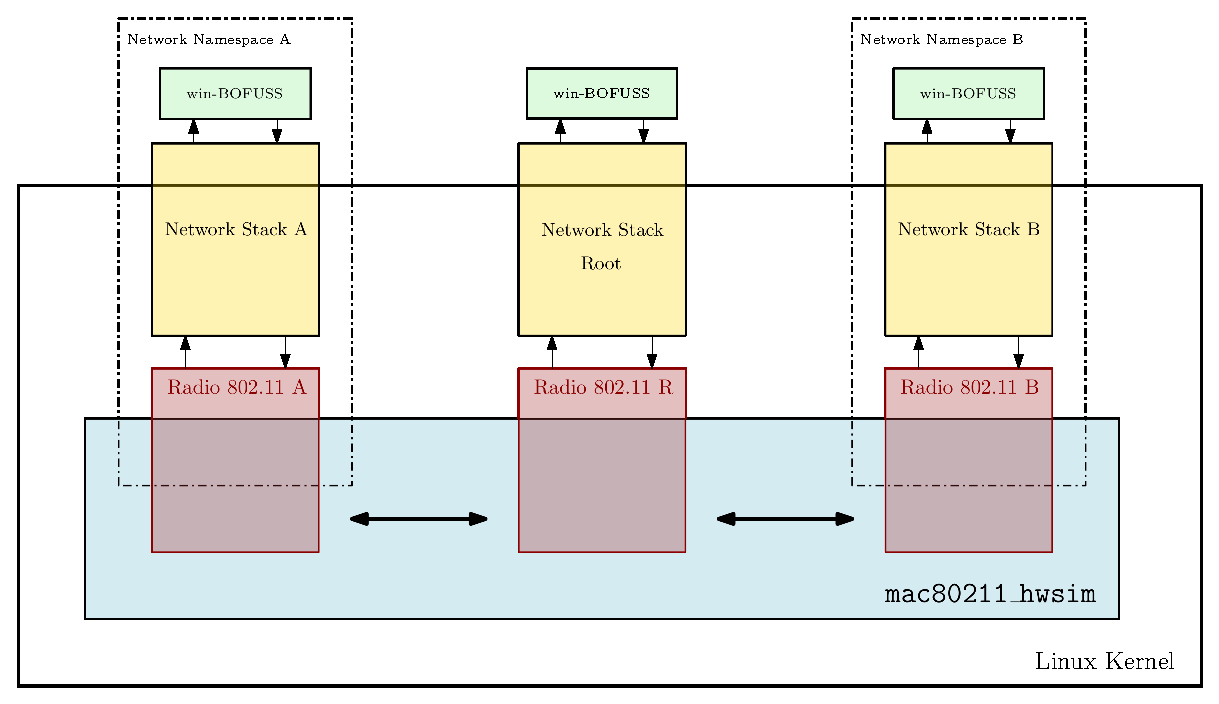
\includegraphics[width=\textwidth]{archivos/img/dev/scenario_eva.eps}
    \caption{Entorno de validación haciendo uso del módulo del Kernel \texttt{mac80211\_hwsim}}
    \label{fig:scenario_eva}
\end{figure}

Cada nodo de la topología se encapsulará en una Network namespace, la cual contendrá una de las radios WiFi emuladas por el módulo del Kernel \texttt{mac80211\_hwsim}. De esta forma se consigue que el tráfico no atraviese de un nodo al nodo raíz directamente, y siga la ruta preestablecida de la topología física emulada. Las radios internamente se verán entre ellas dentro del módulo del Kernel, donde se intercambiarán los mensajes radio, los cuales serán delegados al procesado del \textit{stack} de red que corresponda, para finalmente, ser entregado al programa de espacio de usuario \texttt{win-BOFUSS}\footnote{Técnicamente son dos, el ofdatapath y el ofprotocol}.\\
\\
De esta forma, se podrán replicar escenarios inalámbricos con relativa rapidez, y de una forma sencilla, dado que al utilizar los mismos recursos que Mininet y Mininet-WiFi, se pueden utilizar las herramientas auxiliares a estos para interactuar con el escenario lanzado con el shell script. Se quiere mencionar, que aunque el controlador no aparezca en la Figura \ref{fig:scenario_eva}, este puede correr en cualquiera de las Network namespace que haya en la topología. En nuestro caso, correrá en la Network namespace por defecto, la \textit{root}, donde también correrá el nodo raíz.

\subsection{Comprobación funcional}

En esta subsección se va a realizar una comprobación funcional de la implementación llevada a cabo sobre el \gls{bofus}. Para ello, se va a hacer uso de una topología relativamente sencilla, pero que tiene la conectividad suficiente para ver la operativa real del protocolo IoTorii. La topología está compuesta de 6 nodos, y se ha marcado al nodo \texttt{A} como nodo raíz de la topología, es decir será el nodo que tenga acceso al controlador \gls{sdn}. La topología se puede apreciar en la Figura \ref{fig:topo_eva}.\\
\\
Para poner en marcha el escenario solo se tendrá que lanzar el shell script (Ver sección \ref{sec:estadoArte_github}), y para limpiarlo, como se indicaba anteriormente, se hará uso de la utilidad de Mininet para limpiar los recursos reservados para la emulación de la topología. A continuación, se indica en el bloque de Código \ref{code:eva_scenario} como trabajar con el escenario.

\begin{lstlisting}[language= bash, style=Consola, caption={Puesta en marcha y limpieza del escenario},label=code:eva_scenario]
    # Levantar escenario básico
    sudo ./topo_basic.sh
    
    # Limpiamos
    sudo mn -c
    
\end{lstlisting}
\vspace{0.5cm}

La comprobación funcional consistirá en el estudio y análisis de las tablas de vecinos y \gls{hlm} de cada nodo de la topología. En primera instancia se debatirá como deberá funcionar el protocolo de forma teórica, más adelante se comprobará accediendo a los logs de cada \texttt{win-BOFUSS} el contenido de las tablas de vecinos y de \gls{hlm} para comprobar si el funcionamiento esperado y real coinciden. En esta validación se habría querido poner alguna captura de Wireshark, pero, al no haber programado un disector para el protocolo IoTorii, no será posible apreciar el contenido de los mensajes intercambiados entre los nodos de la topología, solo se verá un campo que indique data con una cadena hexadecimal.\\


% topo eva
\begin{figure}[ht]
    \centering
    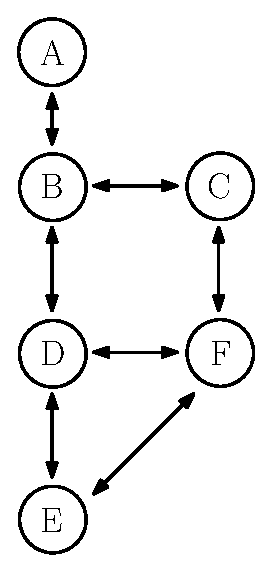
\includegraphics[width=0.42\textwidth]{archivos/img/dev/topo_eva.eps}
    \caption{Topología básica a evaluar el funcionamiento de IoTorii}
    \label{fig:topo_eva}
\end{figure}

Según se ha indicado anteriormente, al trabajar con los mismos recursos que Mininet-WiFi, podremos utilizar herramientas auxiliares que incorporan. Si ya se ha lanzado la topología, y se inicia el núcleo de Mininet-WiFi, pasándole las coordenadas de cada nodo se puede comprobar si el escenario se ha levantado correctamente dibujando la topología. A continuación, en la Figura \ref{fig:topo_val_mininetWifi}, se puede apreciar la topología básica levantada a través de Mininet-WiFi.\\
\\

\begin{figure}[ht]
    \centering
    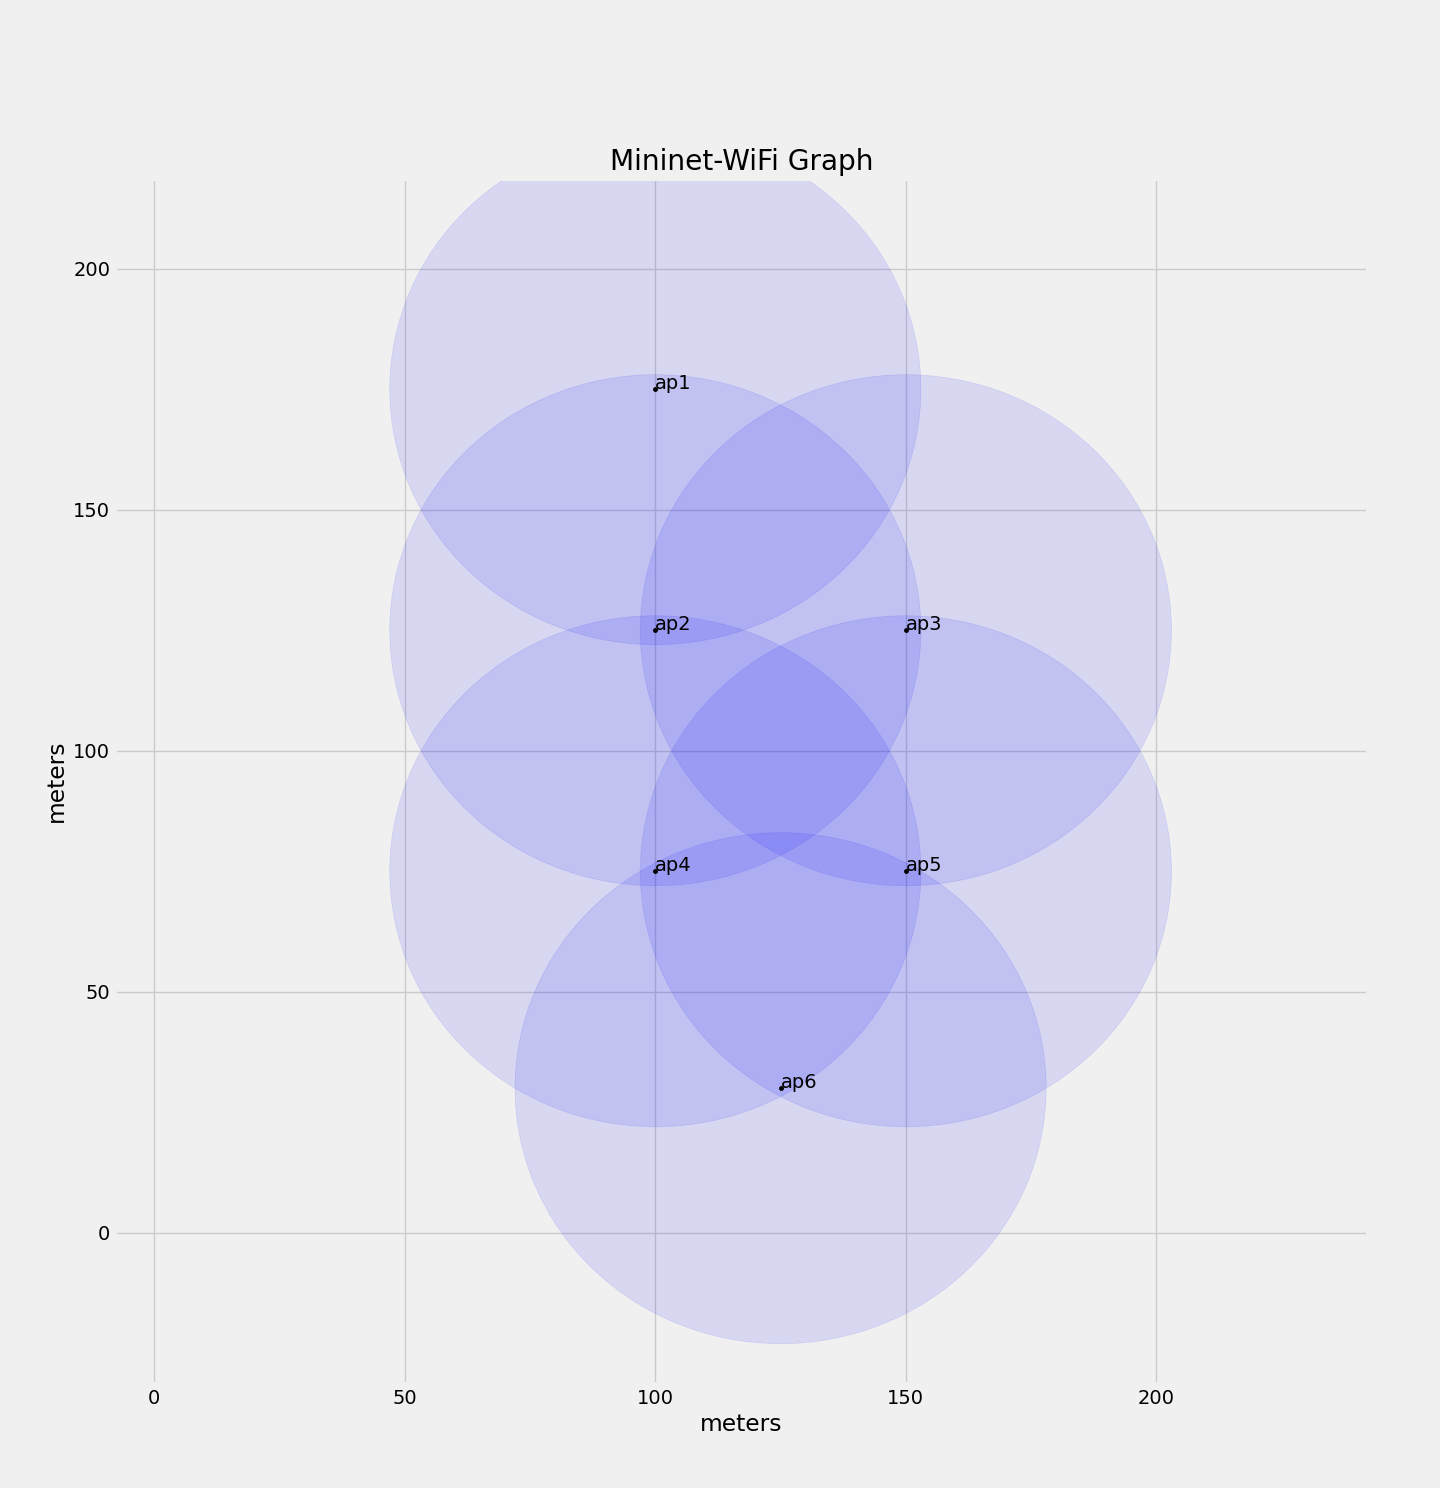
\includegraphics[width=0.8\textwidth]{archivos/img/dev/topo_val_mininetWifi.png}
    \caption{Topología básica representada con el motor de Mininet-WiFi}
    \label{fig:topo_val_mininetWifi}
\end{figure}

Otro problema que se ha encontrado a la hora de emular, es el problema mencionado anteriormente en la memoria en la Sección \ref{subsubsec:problemasmalos}. Cuando se ha intentado emular topologías más grandes, parece que el módulo del Kernel no hace un buen uso de los recursos reservados dado que las interfaces generadas son bloqueadas por el Kernel vía \textit{software}. Por ello, se ha querido demostrar el funcionamiento en una topología sencilla, que funcione de forma sólida y sea fácil de apreciar el funcionamiento del protocolo.

\subsubsection{Tablas de vecinos}

En este punto se va a estudiar las tablas de vecinos para la topología anteriormente presentada, así como la operativa básica de anuncio de vecindad mediante el intercambio de mensajes \textit{Hello}. Recordemos que la condición de vecinos se da siempre y cuando dos nodos se encuentren en rango de señal entre ellos y se hayan notificado respectivamente. Cuando se notifican entre ellos, cada nodo apunta en una tabla los vecinos que tiene, guardando su dirección MAC real junto a un sufijo único. Dicho sufijo puede variar en función de la implementación, en este caso es un contador al uso.\\


% topo hellos
\begin{figure}[ht]
    \centering
    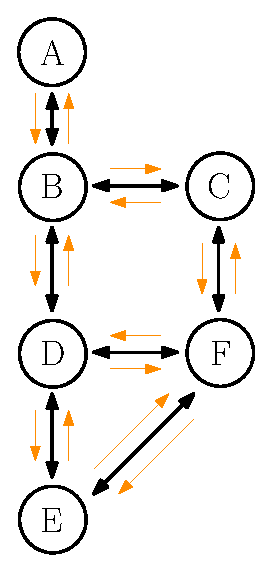
\includegraphics[width=0.4\textwidth]{archivos/img/dev/topo_hellos.eps}
    \caption{Intercambio de mensajes de tipo \textit{Hello} en la topología básica}
    \label{fig:topo_hellos}
\end{figure}

Si nos detenemos a observar la Figura \ref{fig:topo_hellos}, podremos apreciar cómo todos los nodos presentes en la topología generan mensajes del tipo \textit{Hello} únicamente con aquellos nodos que se encuentran dentro de su rango de comunicación. Es importante destacar que la cantidad de mensajes \textit{Hello} generados será directamente proporcional al tamaño de la topología, es decir, a la cantidad de nodos \textit{N} presentes en ella.\\
\\
Esta relación entre la cantidad de mensajes \textit{Hello} y el número de nodos se debe a que cada nodo necesita establecer y mantener un vínculo de conectividad con los demás nodos dentro de su rango. A medida que aumenta el número de nodos en la topología, la complejidad de los mensajes \textit{Hello} también aumenta, ya que cada nodo debe comunicarse con todos los demás nodos que están a su alcance.\\
\\
De esta manera, la generación de mensajes \textit{Hello} se convierte en un mecanismo esencial para mantener una visión actualizada de la topología de la red, permitiendo a los nodos conocer y establecer conexiones con sus vecinos cercanos. Así, la cantidad y el contenido de los mensajes \textit{Hello} desempeñan un papel crítico en la configuración y el funcionamiento adecuado del protocolo en una topología determinada.\\
\\
Observando la topología, ver figura \ref{fig:topo_hello_nodoA_nb} se puede apreciar como el único vecino que tendrá el nodo raíz será el nodo \texttt{B}, por lo que despues de notificarse, el nodo \texttt{A} apuntará al nodo \texttt{B} en su tabla de vecinos, teniendo en cuenta su dirección MAC real, y le asignará un sufijo único que en este caso es un contador que se va incrementando según se descubrenvecinos nuevos.\\

% topo nb - node A
\begin{figure}[ht!]
    \centering
    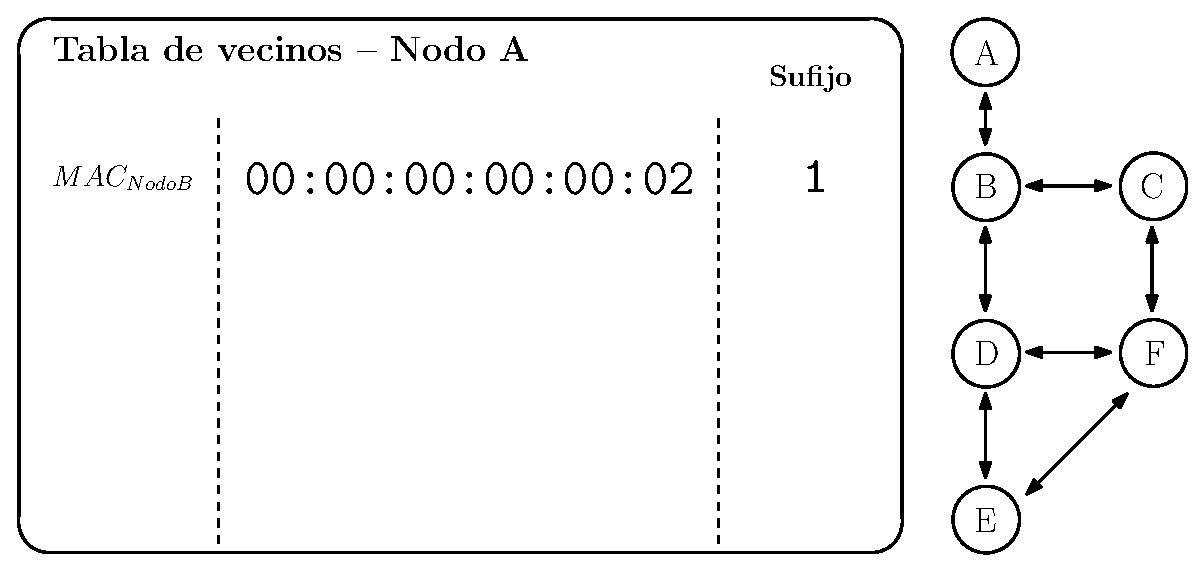
\includegraphics[width=\textwidth]{archivos/img/dev/topo_hello_nodoA_nb.eps}
    \caption{Tabla de vecinos para el nodo \texttt{A}}
    \label{fig:topo_hello_nodoA_nb}
\end{figure}

Si nos fijamos por ejemplo en la tabla de vecinos del nodo \texttt{B}, ver figura \ref{fig:topo_hello_nodoB_nb}, se puede ver como es este caso este nodo tiene como vecinos a los nodos \texttt{[A,C,D]}, por lo que tendrá que generar tres sufijos únicos,\texttt{[1,2,3]}, uno por cada uno de ellos, para después almacenar la MAC real junto a dicho sufijo único.\\

% topo nb - node B
\begin{figure}[ht!]
    \centering
    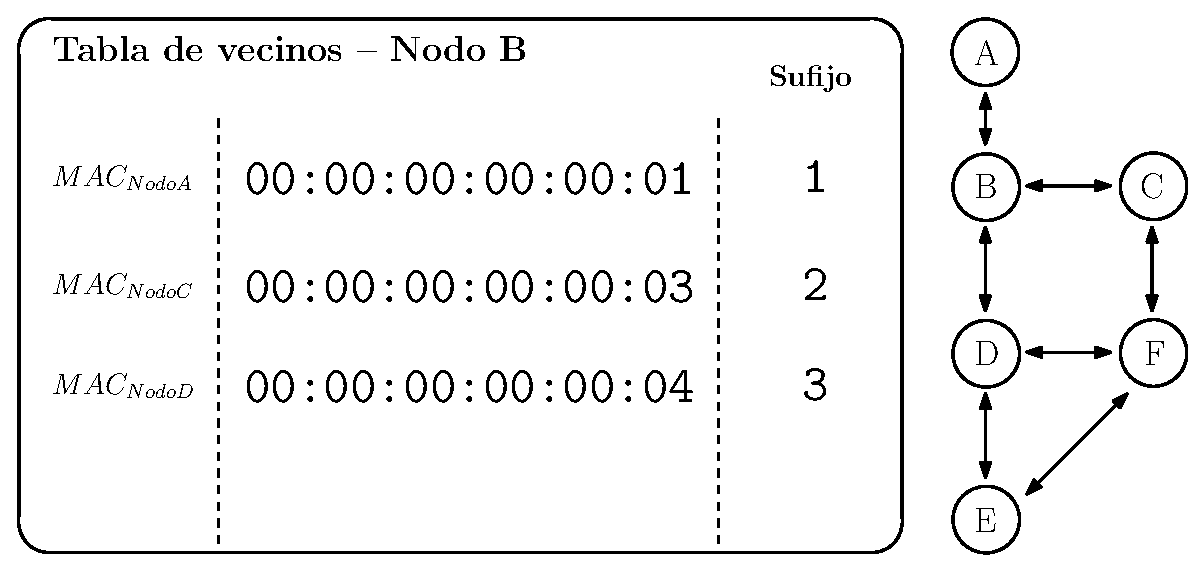
\includegraphics[width=\textwidth]{archivos/img/dev/topo_hello_nodoB_nb.eps}
    \caption{Tabla de vecinos para el nodo \texttt{B}}
    \label{fig:topo_hello_nodoB_nb}
\end{figure}

En cuanto al nodo \texttt{C}, ver Figura \ref{fig:topo_hello_nodoC_nb}, se puede ver en la topología que solo tendrá como vecinos a los nodos \texttt{[B,F]}, por lo que solo hará uso de dos sufijos únicos.\\

% topo nb - node C
\begin{figure}[ht!]
    \centering
    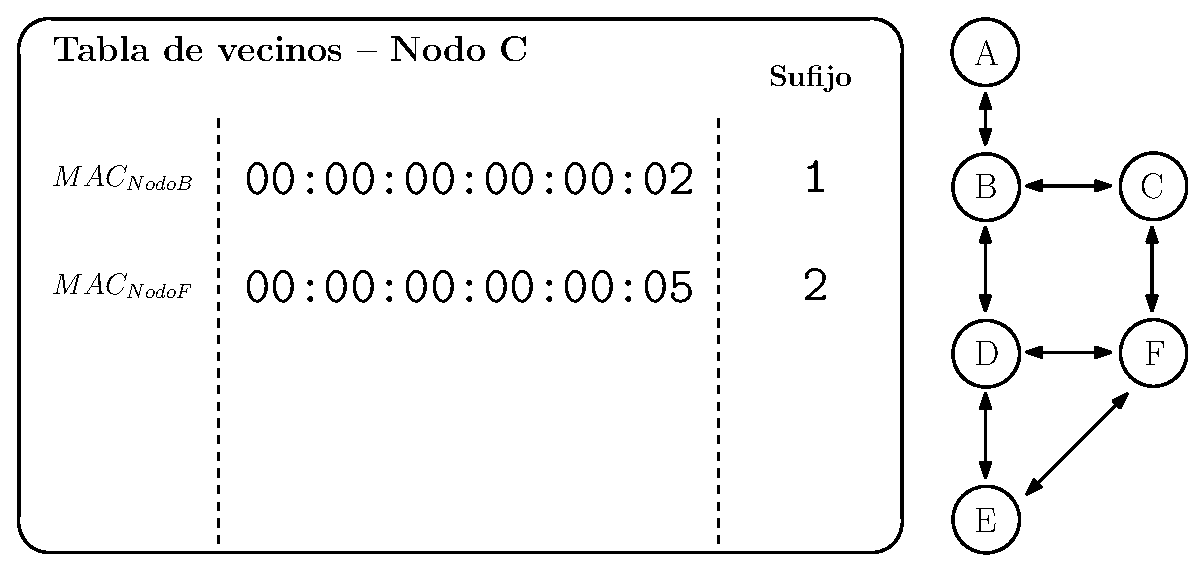
\includegraphics[width=\textwidth]{archivos/img/dev/topo_hello_nodoC_nb.eps}
    \caption{Tabla de vecinos para el nodo \texttt{C}}
    \label{fig:topo_hello_nodoC_nb}
\end{figure}

En cuanto a los nodos \texttt{D}, \texttt{F} y \texttt{E}, ver Figuras \ref{fig:topo_hello_nodoD_nb}, \ref{fig:topo_hello_nodoF_nb} y \ref{fig:topo_hello_nodoE_nb}, se tienen ambos como vecinos y rellenarán sus tablas de vecinos de forma análoga. Mencionar que el nodo \texttt{D}, al igual que el nodo \texttt{B}, es un nodo hiperconectivo de la topología por lo que tendrá bastantes rutas alternativas para alcanzar al nodo \textit{root}.\\


% topo nb - node D
\begin{figure}[ht!]
    \centering
    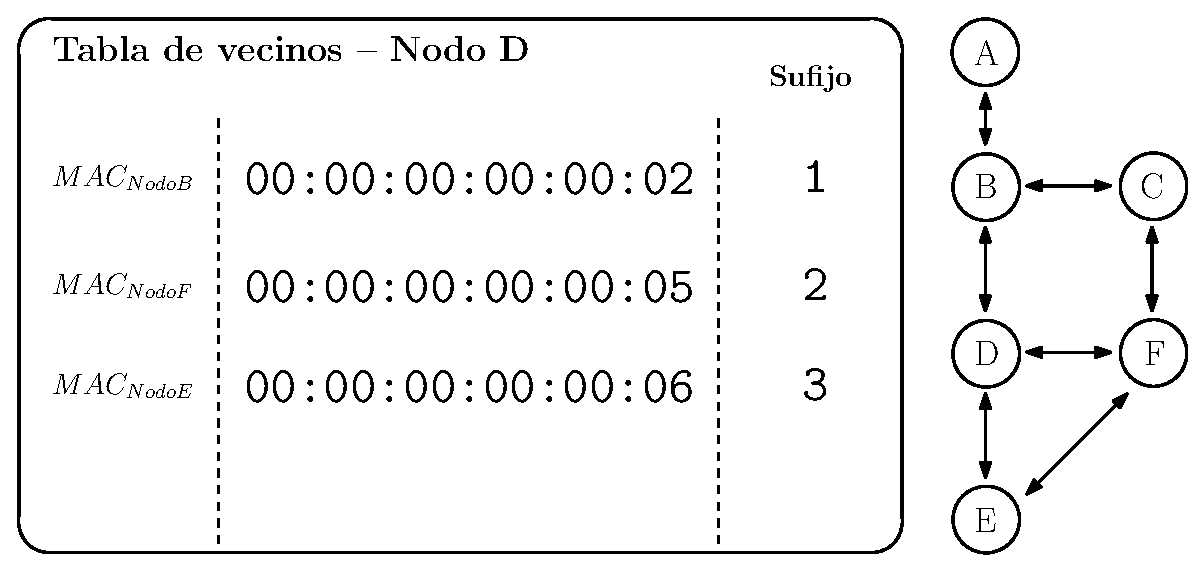
\includegraphics[width=\textwidth]{archivos/img/dev/topo_hello_nodoD_nb.eps}
    \caption{Tabla de vecinos para el nodo \texttt{D}}
    \label{fig:topo_hello_nodoD_nb}
\end{figure}


% topo nb - node E
\begin{figure}[ht!]
    \centering
    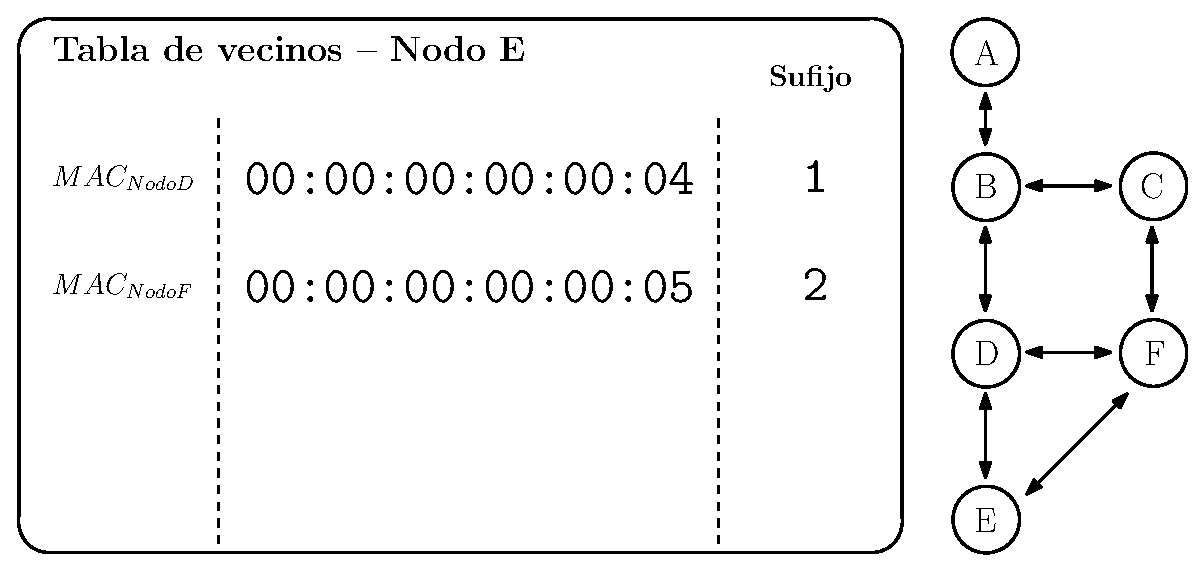
\includegraphics[width=\textwidth]{archivos/img/dev/topo_hello_nodoE_nb.eps}
    \caption{Tabla de vecinos para el nodo \texttt{E}}
    \label{fig:topo_hello_nodoE_nb}
\end{figure}

\newpage


% topo nb - node F
\begin{figure}[ht!]
    \centering
    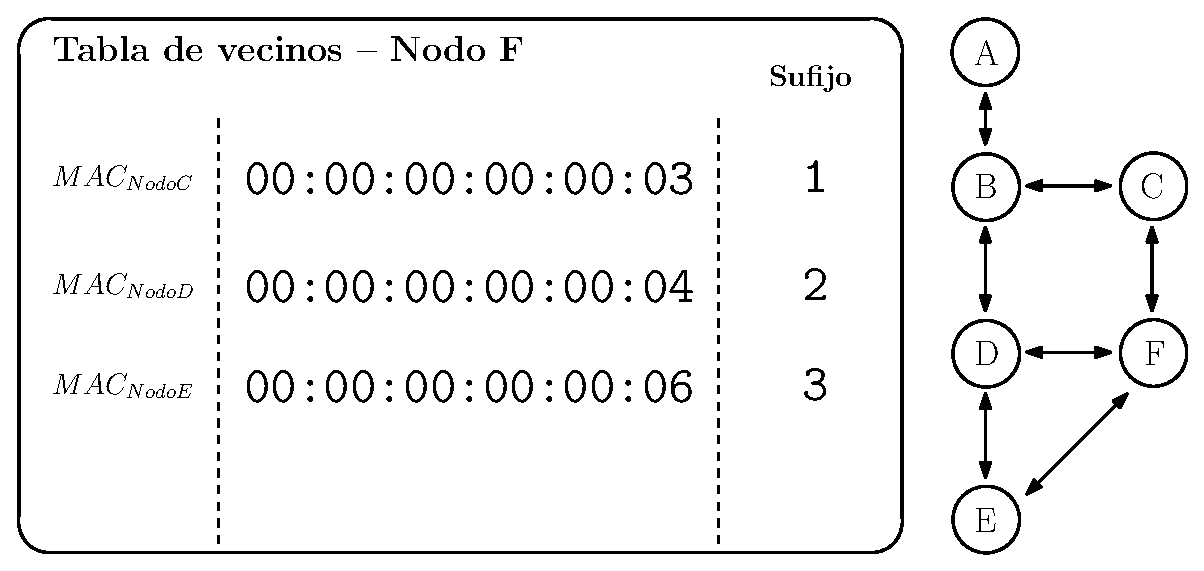
\includegraphics[width=\textwidth]{archivos/img/dev/topo_hello_nodoF_nb.eps}
    \caption{Tabla de vecinos para el nodo \texttt{F}}
    \label{fig:topo_hello_nodoF_nb}
\end{figure}


Hemos examinado detalladamente el comportamiento teórico del proceso de notificación de vecindad entre los nodos de la topología. Hemos explorado cómo los mensajes \textit{Hello} permiten a los nodos establecer y mantener conexiones con sus vecinos cercanos, creando una visión actualizada de la estructura de la red.\\
\\
Sin embargo, la comprobación teórica por sí sola no basta para garantizar la solidez y efectividad de la implementación. Es por ello que ahora nos adentraremos en la fase de contrastar este comportamiento teórico con el funcionamiento real de la misma topología, la cual hemos emulado con las condiciones reales de una red inalámbrica. Esto nos permitirá evaluar el desempeño y la estabilidad de la implementación en un entorno pseudo-real. Analizaremos el comportamiento de los nodos en tiempo real, observando cómo interactúan entre sí y si la generación y recepción de mensajes \textit{Hello} se desarrolla de acuerdo con lo esperado. Mediante este enfoque, buscaremos obtener conclusiones sólidas y fiables sobre la capacidad del protocolo para adaptarse a cambios en la topología, como la aparición o desaparición de nodos y enlaces.\\
\\
Para ello, se ha levantado la topología según se ha explicado en el bloque de Código \ref{code:eva_scenario}, y se han abierto los seis ficheros de log asociados a las tablas de vecinos de cada nodo de la topología (\texttt{/tmp/ap\_X\_nb.log}). Como se puede apreciar en la Figura \ref{fig:nb_real}, todas las tablas de vecinos coinciden con las tablas que se han ido analizando poco a poco de forma teórica, por lo que se asume que esta parte de la implementación se ha realizado satisfactoriamente.

% logs nb tables
\begin{sidewaysfigure}[htbp]
    \begin{center}
        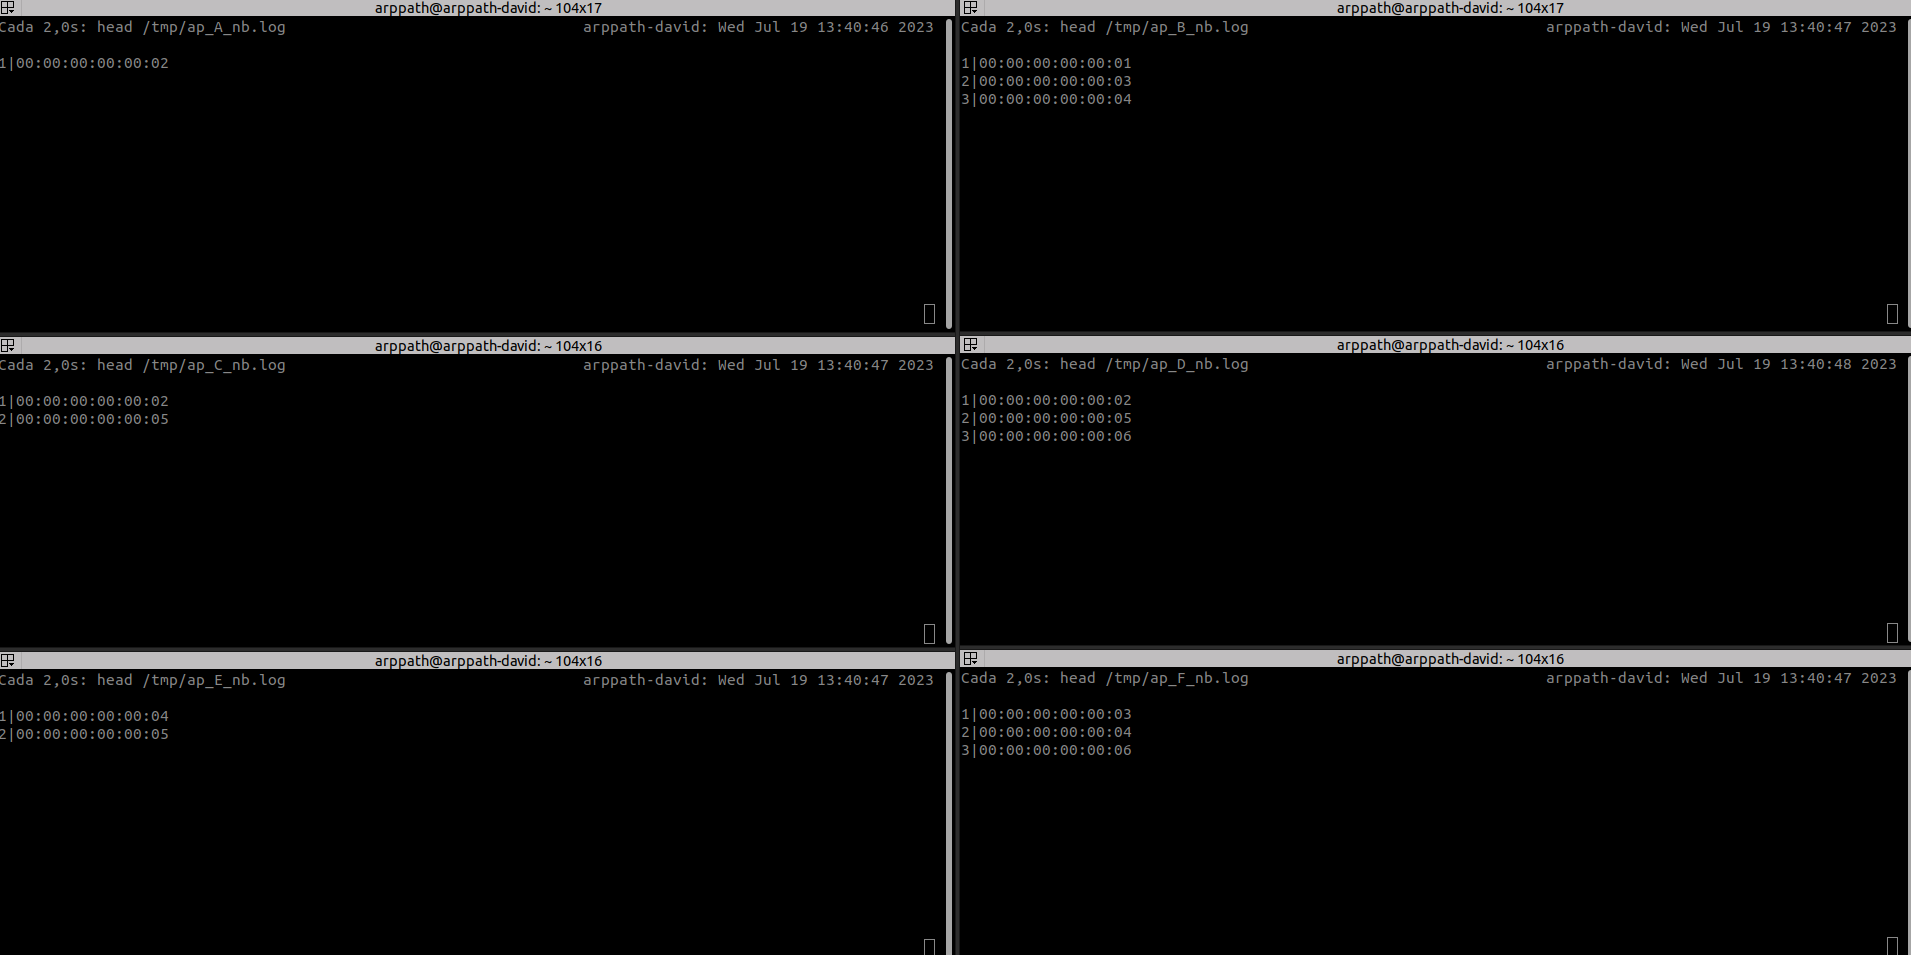
\includegraphics[width=\textwidth]{archivos/img/dev/nb_real.png}
        \caption{Tabla de vecinos extraídas de los logs de los \textit{software switches}}
        \label{fig:nb_real}
    \end{center}
\end{sidewaysfigure}


\subsubsection{Tablas \glsentryshort{hlm}}

En este punto se van a estudiar las tablas de rutas conocidas como \gls{hlm}, así como la operativa básica de anuncio de rutas al nodo raíz mediante el intercambio de mensajes \textit{SetHLMAC}. Recordemos que para que un nodo genere un mensaje genere un mensaje de \textit{SetHLMAC}, antes ha tenido que recibir una \gls{hlm}, y tener vecinos para intercambiarla. Cuando se notifica una ruta aun vecino, va la \gls{hlm} recibida más un sufijo único del vecino. De esta forma la \gls{hlm} aumenta en un nivel más.\\
\\
A continuación, en la Figura \ref{fig:topo_sethlmac}, se ha intentado ilustrar todo el proceso de difusión de estos mensajes \textit{SetHLMAC} a lo largo de la topología. Se han incluido cuatro \textit{snapshots}, siguiendo un orden cronológico de izquierda a derecha y de arriba abajo. Es importante señalar que aunque en esta figura se hayan representado así el intercambio de mensajes, no tiene por qué realizarse en ese mismo orden. Esto es así porque en la realidad hay que tener en cuenta latencias y tiempos de procesamiento.\\
\\
Volviendo a la Figura \ref{fig:topo_sethlmac}, se puede apreciar como en primera instancia la primera oleada de difusión empieza por el nodo \texttt{A}, generando la \gls{hlm} con valor \texttt{1}, la cual será difundida a todos los vecinos de \texttt{A}, que en este caso es el nodo \texttt{B}. Si nos fijamos en la tabla de vecinos del nodo \texttt{A}, podemos ver como el nodo \texttt{B} tiene el sufijo único con valor \texttt{1}. Por tanto, la \gls{hlm} que le llegará al nodo \texttt{B} será \texttt{1.1}. Este proceso se lleva a cabo de forma análoga por toda la topología, el nodo \texttt{B}, una vez que le llega la nueva \gls{hlm} con valor \texttt{1.1} procederá a difundirla a todos sus vecinos, que en este caso son el nodo \texttt{C} y \texttt{D} respectivamente. El nodo \texttt{B} comprobará su tabla de vecinos en busca de los  nodos \texttt{C} y \texttt{D}, y generará las \gls{hlm} \texttt{1.1.3} y \texttt{1.1.2}.\\
\\
Se quiere mencionar que hay algunas \gls{hlm} que no se difundían para evitar bucles en la topología.  La condición de ser una \gls{hlm} válida es la de no ser hija de una ya almacenada en la tabla de rutas de un nodo en cuestión. Por ejemplo, si tenemos la ruta \texttt{1.1.2}, todas las rutas del tipo \texttt{1.1.2.X.Y} serán descartadas.\\
\\
Otro detalle que se quiere mencionar de la implementación, es el criterio que se ha seguido para elegir una ruta al nodo raíz frente a otras. En este caso se marca como \gls{hlm} activa aquella que llegue antes al nodo. Se pueden establecer muchos criterior para tomar esta decisión, desarrollando una función objteivo y evaluar cada ruta en base a unos criterios, pero en este caso, se va a coger la primera ruta que llegue que se entenderá que es aquella ruta más rapida en alcanzar al \textit{root}.\\

\newpage
% topo difu hlmac
\begin{figure}[ht]
    \centering
    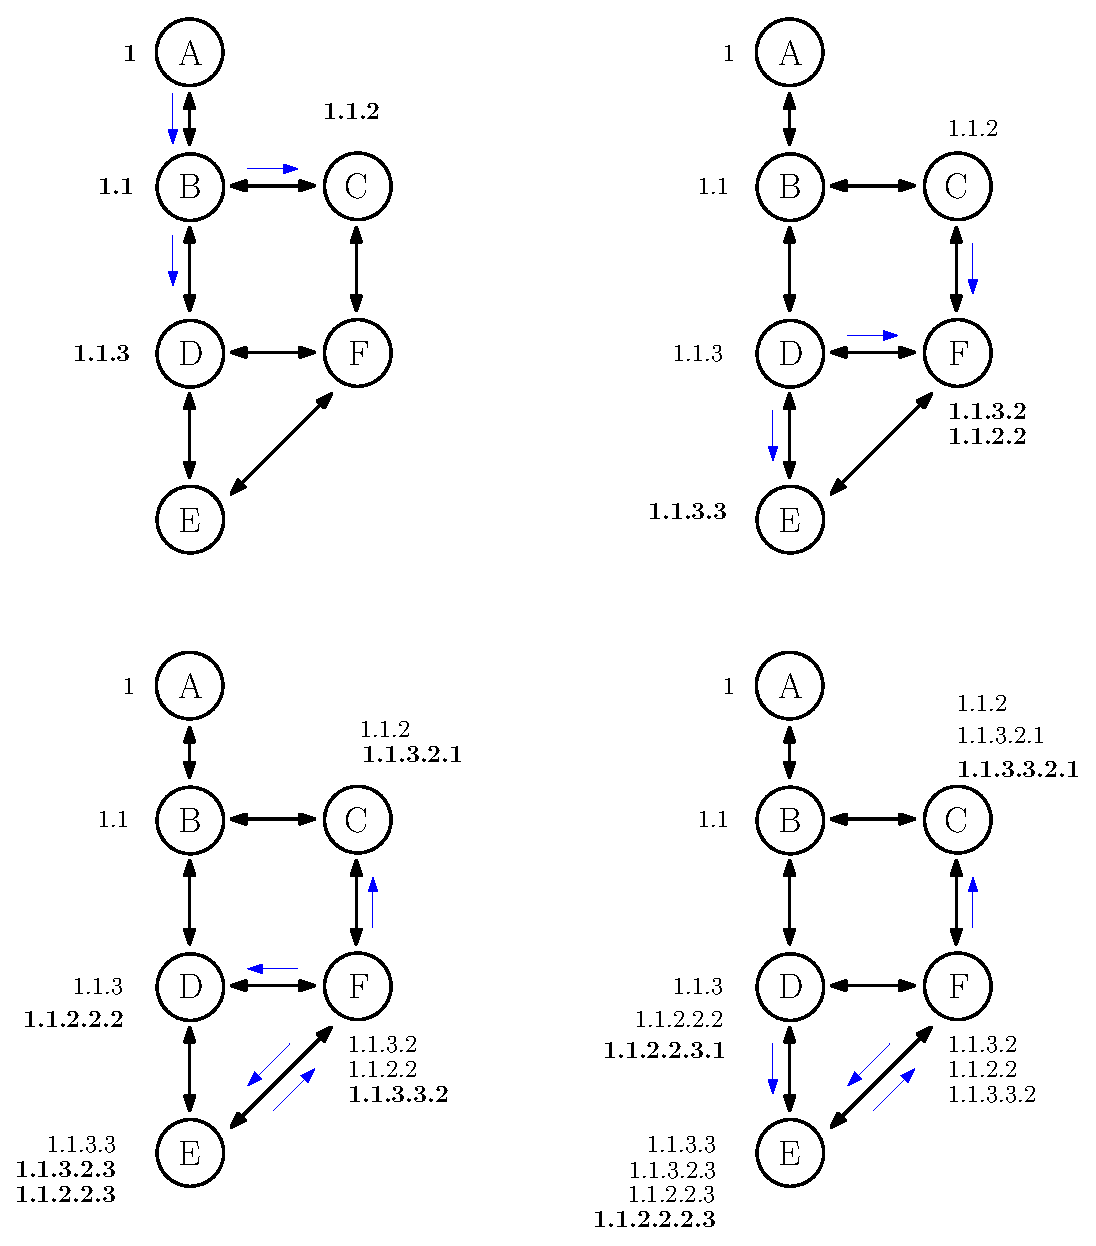
\includegraphics[width=\textwidth]{archivos/img/dev/topo_sethlmac.eps}
    \caption{Proceso de difusión de mensajes de tipo \textit{SetHLMAC} en la topología básica}
    \label{fig:topo_sethlmac}
\end{figure}
\newpage
% logs hlmac tables
\begin{sidewaysfigure}[htbp]
    \begin{center}
        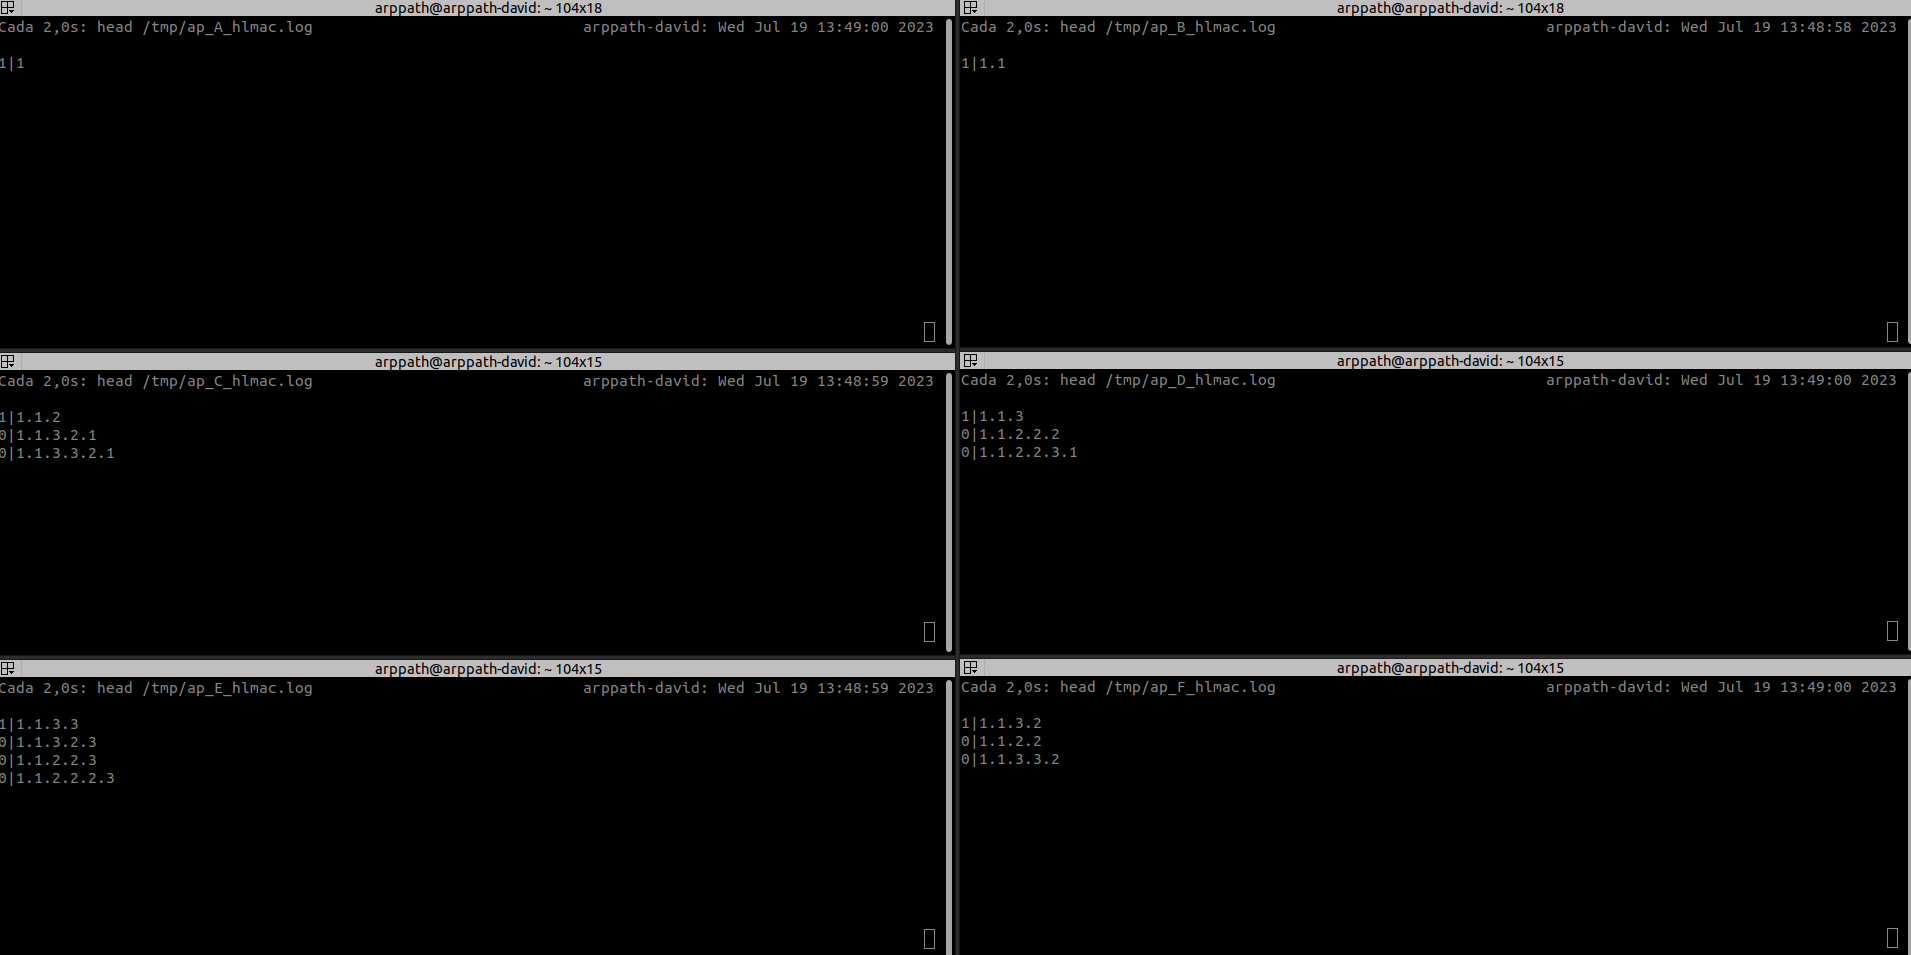
\includegraphics[width=\textwidth]{archivos/img/dev/hlmac_real.png}
        \caption{Tabla de HLMAC extraídas de los logs de los \textit{software switches}}
        \label{fig:hlmac_real}
    \end{center}
\end{sidewaysfigure}
\newpage
Si nos fijamos en la comprobación en real del escenario emulado, todas las tablas de rutas \gls{hlm} coinciden por lo que se da por satisfactoria la comprobación funcional del protocolo. La comprobación en real se ha llevado a cabo consultando los ficheros de logs generados por el \texttt{win-BOFUSS} en el path \texttt{/tmp/ap\_X\_hlmac.log}. El formato de dichos ficheros de log es el siguiente, \texttt{flag | HLMAC }. Por lo que se puede apreciar aquellas \gls{hlm} que llegan antes al nodo serán marcadas como rutas activas al nodo raíz. Una vez difundidas las etiquetas, y marcada al menos una por nodo, se puede apreciar como a partir de la topología física inalámbrica se puede obtener la topología lógica.\\
\\
En la Figura \ref{fig:topo_logic}, podemos observar la topología física que ha sido estudiada en la sección anterior, compuesta por un total de 6 nodos. Tras difundir las etiquetas, hemos aplicado el criterio basado en la ruta más rapida, lo que ha permitido que cada nodo de la topología obtenga su respectiva \gls{hlm}, como se muestra en la figura. Una vez que todos los nodos han adquirido sus \gls{hlm} es probable que algunos enlaces de la topología queden en desuso, ya que no existirá ninguna etiqueta que haga uso de dichos enlaces. Esto se debe a que el proceso de determinar las \gls{hlm} permite a los nodos seleccionar rutas óptimas hacia el nodo raíz, lo que podría resultar en que algunos enlaces no sean necesarios. Es importante resaltar que este proceso de selección de rutas y asignación de \gls{hlm} tiene un impacto significativo en la eficiencia y utilización de los enlaces en la topología. Aquellos enlaces que no sean utilizados quedan en desuso, lo que podría liberar recursos y mejorar la capacidad de la red para adaptarse a cambios en la topología.\\
\\
Si consideramos todas las $HLMAC_{active}$ de los nodos en la topología, podemos definir una topología lógica que contiene todos los nodos de la topología física pero solo un subconjunto de los enlaces presentes en dicha topología física. Este proceso de establecer la topología lógica puede ser formulado utilizando un grafo $G \: = \: (\mathcal{N}, \mathcal{L})$, donde $\mathcal{N}$ es un conjunto de $N$ nodos y $\mathcal{L} \subseteq \{\{i,j\} \: | \: i,j \in \mathcal{N} \: and \: i \neq j\}$ es un conjunto de enlaces, cada uno compuesto por un par desordenado de nodos (es decir, cada enlace conecta dos nodos distintos).\\
\\
Al obtener la topología lógica, se crea un subgrafo $G' \: = \: (\mathcal{N}', \mathcal{L}')$ en el que se cumple que $\mathcal{N}' \subseteq \mathcal{N}$ y $\mathcal{L}' \subseteq \mathcal{L}$. Es decir, la topología lógica contiene un subconjunto de los nodos y un subconjunto de los enlaces de la topología física. Sin embargo, se debe destacar que en este caso, los nodos son idénticos en ambas topologías, lo que se expresa mediante la relación de igualdad para los nodos. Esto significa que todos los nodos en la topología lógica $\mathcal{N}'$ son iguales a los nodos en la topología física $\mathcal{N}$. Es decir, si $a_{i} \in \mathcal{N}$ y $b_{i} \in \mathcal{N}'$, donde $0 \leq i \leq N$, se cumple que para cada nodo $a_{i}$ y su correspondiente nodo en la topología lógica $b_{i}$, se tiene que $a_{i} \: = \: b_{i}$.
% topo logic vsr fisica
\begin{figure}[ht]
    \centering
    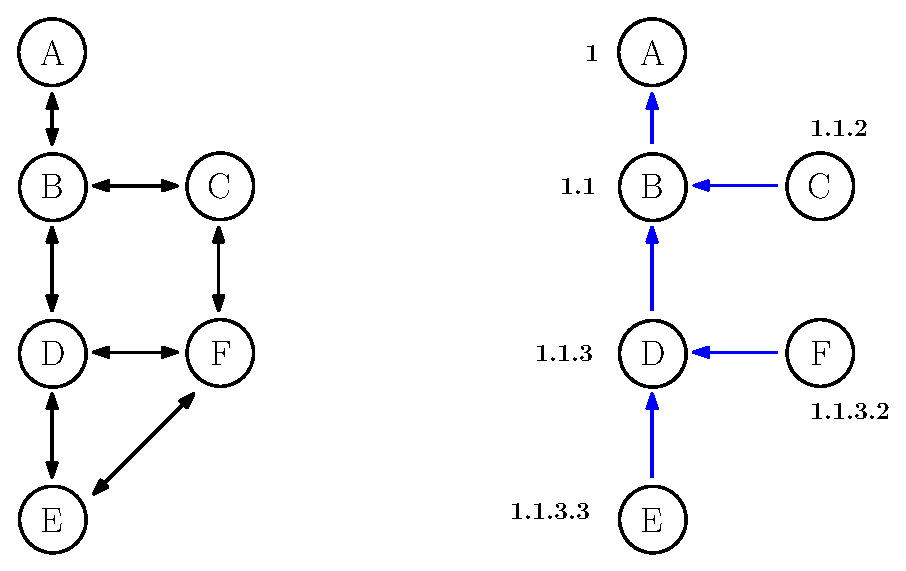
\includegraphics[width=\textwidth]{archivos/img/dev/topo_logic.eps}
    \caption{Establecimiento de la topología lógica}
    \label{fig:topo_logic}
\end{figure}

% Lets see tomorrow
%\subsection{Comprobación cuantitativa}